\section{Aufbau Bot}
\label{sec:module.AufbauBot}


\subsection{Klasse Bot}
\label{sec:module.Bot.Bot}

\begin{figure}[H]
\centering
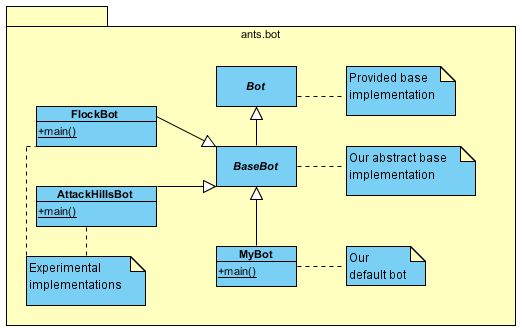
\includegraphics[width=0.7\textwidth]{91_bilder/antsBot}
\caption{Vererbung der Bots wobei auf Stufe impl (Implementation) nur MyBot verwendet wird.}
\label{fig:antsBot}
\end{figure}

Als Basis f�r unsere Bot Implementation haben wir den Beispiel-Bot (Klasse Bot.java) verwendet, der im Java-Starter-Package enthalten ist, das von der AI-Challenge-Website heruntergeladen werden kann. Dieser erbt von den Klassen AbstractSystemInputReader und AbstractSystemInputParser, die die Interaktion mit der Spiele-Engine �ber die System-Input/Output Streams kapseln. F�r eine optimierte L�sung k�nnte der Bot auch angepasst werden, indem er selber auf die Streams zugreift. Im Rahmen dieser Arbeit erschien uns das aber noch nicht n�tig. Die Klasse Bot.java dient als Grundlage f�r die Klasse BaseBot, welcher wiederum Grundlage ist f�r die Finale Klasse MyBot.java.



\subsection{BaseBot}
\label{sec:module.Bot.BaseBot}

Die abstrakte Klasse BaseBot erbt vom Bot. Hier haben wird die Struktur unseres Spielzuges definiert.

\subsection{Ablauf eines Zugs} 
\label{sec:implementation.Bot.Turn}

\begin{figure}[H]
\centering
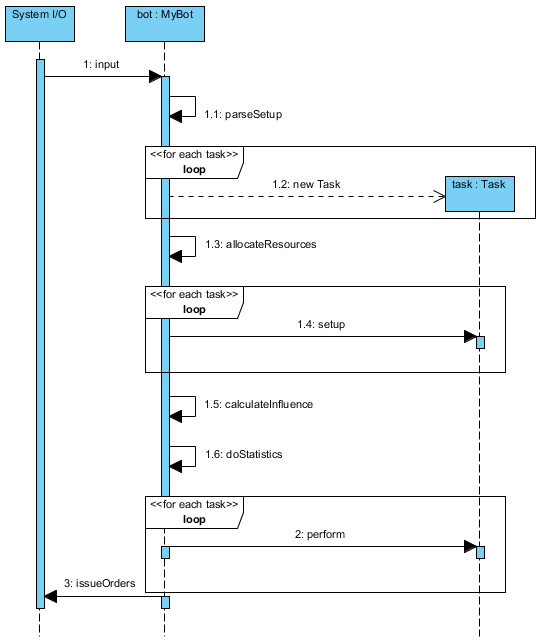
\includegraphics[width=0.9\textwidth]{91_bilder/FirstTurn}
\caption{Ablauf des ersten Zugs des Spiels}
\label{fig:firstTurn}
\end{figure}

\begin{figure}[H]
\centering
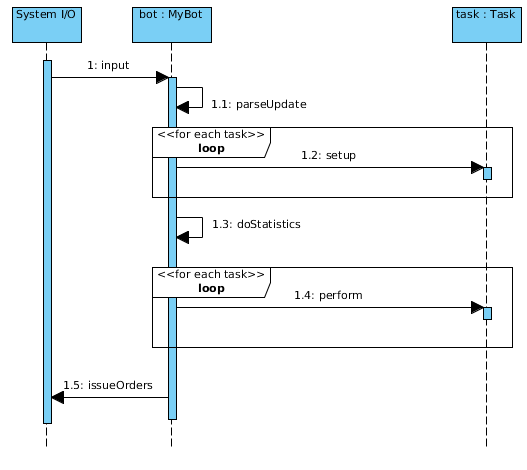
\includegraphics[width=0.9\textwidth]{91_bilder/Turn}
\caption{Ablauf der weiteren Z�ge des Spiels}
\label{fig:turn}
\end{figure}


TODO calculateInfluence() fehlt 

Abbildung \ref{fig:firstTurn} zeigt den Ablauf des ersten Zugs, w�hrend Abbildung \ref{fig:turn} den Ablauf aller weiteren Z�ge zeigt. 

Jeder Zug beginnt mit dem Einlesen des Inputs vom SystemInputStream. Wenn der Bot das Signal ''READY`` (1. Zug) oder ''GO`` (alle weiteren Z�ge) erh�lt, kann er den gesammelten Input verarbeiten (Methode parseSetup() resp. parseUpdate()). Danach wird die eigentliche Logik des Bots in der Methode doTurn(...) ausgef�hrt.

Im 1. Zug werden dabei Instanzen der Tasks erstellt. Abgesehen davon unterscheidet sich der 1. Zug von diesem Punkt an nicht mehr von allen nachfolgenden Z�gen. Die Tasks werden vorbereitet. (Aufruf der jeweiligen setup() Methode. Danach werden einige statistische Werte aktualisiert und in jedem 10. Zug auch geloggt. Dann werden die Tasks in der definierten Reihenfolge aufgerufen. Hier wird der L�wenanteil der Zeit verbracht, denn die Tasks enthalten die eigentliche Logik unserer Ameisen.

Zum Schluss werden dann mit issueOrders() die Z�ge der Ameisen �ber den SystemOutputStream an die Spielengine �bergeben. Im Code sieht das ganze folgendermassen aus.

\begin{verbatim}
@Override
/*
 * This is the main loop of the bot. All the actual work is
 * done in the tasks that are executed in the order they are defined.
 */
public void doTurn() {
		// write current turn number, ants amount into the log file.
	addTurnSummaryToLogfiles();
		// new calculation of the influence map
	calculateInfluence();
		// write some statistics about our population
	doStatistics();
		// initialize the task (abstract method) must be implemented by the inherited class
	initTasks();
		// execute all task (main work to do here)
	executeTask();
		// write all orders to the output stream
	Ants.getOrders().issueOrders();
		// log all ants which didn't get a job.
	logUnemployedAnts();
}
\end{verbatim}


\subsection{MyBot}
\label{sec:module.Bot.MyBot}

Wie bereits erw�hnt ist die Methode initTasks() in BaseBot abstrakt und muss von MyBot implementiert werden. InitTasks() definiert welche Tasks, oder besser gesagt F�higkeiten der Bot hat. Dies wurde ausgelagert, da nicht nur MyBot von BaseBot erbt, sondern auch weiter Bots die wir zu Testzwecken erstellt haben um nur gewisse Funktionalit�ten zu testen. (Siehe dazu \ref{sec:testCenter.Testbots}) Weiter wird in MyBot initLogging(...) aufgerufen. Hier definieren wir welche Logkategorien mit welchem Loglevel ins Logfile geschrieben werden. Mehr zum Thema Logging ist im Kapitel Logging zu finden. Je nach Modul das gerade getestet wird k�nnen die Anzahl Logeintr�ge justiert werden.\newline
MyBot initialisiert folgende Tasks; es sind die Tasks die sich w�hrend der Arbeit bew�hrt haben. Die detaillierte Beschreibung der Tasks ist im Kapitel \ref{sec:module.Tasks} zu finden.

\begin{itemize}
		\item GatherFoodTask
		\item AttackHillsTask
		\item DefendHillTask
		\item ExploreTask
		\item ClearHillTask
		\item CombatTask
		\item ClusteringTask
\end{itemize}